\section{Simulation Types}

Because simulation is quite a popular way to program, a lot of different simulation types exist. In this section, we will focus on describing continuous simulation, discrete event-based simulation and agent-based simulation. These three types of simulation are the ones that most closely fit the needs for our project the most, as will be made clear in their following descriptions. The goal for this section is to choose the ideal simulation type for our needs, as well as properly defend our final choice.

\subsection{Continuous Simulation}
A continuous simulation will continuously, "in real time", output the results that the simulation calculates. The results are more accurately the values and systems the simulation has to work with. This means that the simulation will process the algorithms and display the results simultaneously, and not in intervals like event-based simulation described later \citep{howard_what_2020}.

An example of continuous simulation could be video games. In a game, the program or simulation will continuously look for input from the player, while calculating every other aspect the game's real-time progression. This could be a day and night cycle, what other characters behaviour should be, or as simple as what music to play at a given moment \citep{howard_what_2020}.

In short, a continuous simulation outputs results continuously. However, it is difficult to output data in intervals, which is necessary for documenting daily updates in spread of illness. In a similar vein, the continuous simulation type depends on differential equations, which will not be necessary for this project. 

\subsection{Agent-based Simulation}
Agent-based simulation is a type of simulation which simulates individual agents and how these agents can have an effect on the system the agent is part of. These kinds of simulation can be used to study things like social and economic systems. An example of this kind of simulation would be to analyse floor traffic in a shop \citep{howard_what_2020}. -

Agent based simulation would focus on the individuals in the population and their effect on the system (in connection to the spread of a virus). Therefore, it is not ideal for this project, since we are interested in seeing the effect of the system itself.

\subsection{SIR-based Simulation}\label{sec: SIR-based simulation}
The SIR model is a commonly used mathematical model which can approximate the spread of a virus during a pandemic or epidemic. In the SIR model, population is assumed to be a fixed number \textit{N}, which is divided into three groups, susceptible(\textit{S}), infected(\textit{I}) and Removed/Recovered(\textit{R}), where it does not take in to account the amount of people dying. This is where the name, SIR, comes from. These groups are described by three coupled differential equations. When a person leaves one group, they are joining another one, so there can be kept track of every subject in the population \citep{smith_sir_2016}. The SIR model can be used both in discrete-event simulation and in continuous simulation. 

Again, as described above, the only difference is that the continuous simulation will send results continuously and discrete-event based will output in intervals. For the spread of a disease these intervals would most likely be once every day, week or month, depending on the time-span of the simulation \citep{ozmen_analyzing_2016}. The SIR model is the most basic model for a simulation within the epidemiological field. So the SIR model is ideal when dealing with simulating a disease like COVID-19. This also why a SIR-based simulation is the inspiration for our final mode. Unfortunately, it does not quite cover our needs, which leads us to the last simulation type, the discrete event-based simulation.


%It also helps see faults in our simulation, if there are any individuals missing at the end of the simulation, then we know there is a fault in the code.


\subsection{Discrete Event-based Simulation}
A discrete event simulation is a type of simulation that simulates the whole program continuously, but will output the results at predefined intervals. These can be at specific time stamps or only when changes happen \citep{howard_what_2020}.
\begin{figure}[H]
    \centering
    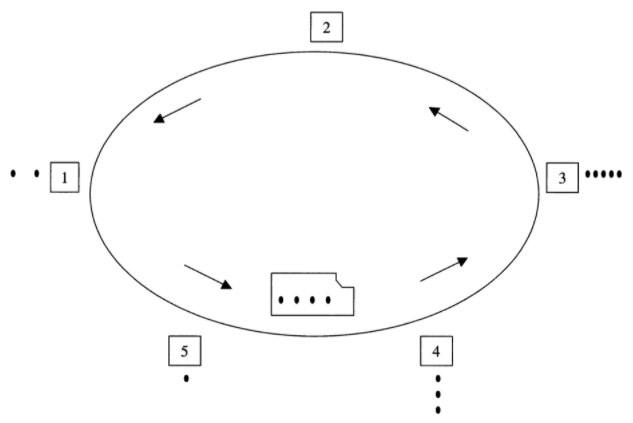
\includegraphics[width=0.75\textwidth]{0_billeder/BusModel.png}
    \caption{Bus Model \citep{fishman_discrete-event_2013}}
    \label{fig:Bus Model}
\end{figure}

Discrete event-based simulation can be looked at like a bus route in figure \ref{fig:Bus Model}. If you were to count the number of passengers on a bus, there would be no need to continuously count them when the bus is driving, as the only time the number of passengers would change is when the bus stops at a bus stop. A simulation of the same bus route would continuously calculate the amount of passengers getting off the bus and the amount of people waiting for the bus. However the simulation would only output the amount of passengers in the bus once every stop \citep{fishman_discrete-event_2013}. 

For simulating the spread of COVID-19 this simulating type is ideal, because our goal is to get a status every day, of how many have been infected, recovered etc. So in our simulation the "bus stop" is every passing day, and here the current status will be output. Therefore, while our simulation is inspired by the SIR-model, the foundation of the code is based on a discrete event-based simulation.

